\documentclass{beamer}
\usetheme{Berkeley}
\usecolortheme{crane}

%\usepackage{default}
\usepackage[utf8]{inputenc} 
\usepackage[english, ngerman]{babel}
\usepackage{xcolor}
\usepackage{epstopdf}
\usepackage{listings}
\lstdefinestyle{C}{
  belowcaptionskip=1\baselineskip,
  breaklines=true,
  frame=L,
  xleftmargin=\parindent,
  language=C,
  showstringspaces=false,
  basicstyle=\footnotesize\ttfamily,
  keywordstyle=\bfseries\color{green!40!black},
  commentstyle=\itshape\color{purple!40!black},
  identifierstyle=\color{blue},
  stringstyle=\color{orange},
  numberstyle=\ttfamily\tiny
}


\title[Monte Carlo]{Die Monte Carlo Methode}
\author[Amiet, Badertscher]{Dorian Amiet, Hannes Badertscher}
\date [MathSem II, FS14]{MathSem II, \today}

% Aufzählungen immer schrittweise zeigen:
\beamerdefaultoverlayspecification{<+->}

% Gliederung am Anfang jedes Unterabschnittes anzeigen:
\AtBeginSection[]
{
  \begin{frame}<beamer>
    \frametitle{Gliederung}
    \tableofcontents[currentsection]
  \end{frame}
}

\begin{document}

\begin{frame}
	\titlepage
\end{frame}
	
\section[Einführung]{Einführung in die Monte Carlo Methode}
\begin{frame}{Einführung in die Monte Carlo Methode}
	Stanisław Marcin Ulam, 1946 
	\begin{itemize}
	\item<1-> Numerische Integration
	\item<1-> Simulation von dynamischen Prozessen
	\item<1-> Simulation von Gleichgewichtszuständen
	\item<1-> Statistische Untersuchung von Zufallsverteilungen
	\end{itemize}
\end{frame}

\section{Numerische Integration}
\begin{frame}{Numerische Integration}

	\begin{minipage}{5cm}
		\includegraphics[width=5cm]{images/kreis_hitmiss.eps}
	\end{minipage}
	\begin{minipage}{5cm}
		\begin{itemize}
		\item<1-> $A_{\text{Kreis}} = \pi r^{2}$
		\item<1-> $A_{\text{Quadrat}} = 4r^2$
		\item<1-> $\hat{\pi} = \frac{A_{\text{Kreis}}}{r^2} = 4 \frac{A_{\text{Kreis}}}{A_{\text{Quadrat}}}$
		\item<1-> $x^2 + y^2 \leq r$
		\end{itemize}
	\end{minipage}
\end{frame}

\subsection{Abschätzung des Wertes von Pi}

\section[Implementation]{Implementation Pi}
\begin{frame}{Implementation}
	\begin{itemize}
		\item Implementation in C: Just do it!
		\item Parallelisierung: perfekt für OpenCL:
			\begin{itemize}
				\item<3-> CPU: Alles initialisieren, Resultat berechnen.
				\item<3-> GPU: Einzelne Punkte berechnen.
			\end{itemize}
	\end{itemize}
\end{frame}
\begin{frame}{Implementation}
	\begin{itemize}
		\item Aufteilung: $N$ Punkte $=$ $N$ Worker.
		\item Zufallszahlen auf GPU? Worker-ID als Seed? \\
		$\rightarrow$ von CPU übergeben. Nachteil: nicht parallel!
		\item Summe und Resultat auf CPU berechnen.
	\end{itemize}
\end{frame}

\begin{frame}{Rechenaufwand}
	Implementation in C:
	\begin{figure}
		\centering
		\includegraphics[width=7cm]{images/Berechnungszeit_C.eps}
	\end{figure}
	11.863 Mio. Berechnungen pro Sec.
\end{frame}
\begin{frame}{Rechenaufwand}
	Implementation in OpenCL:
	\begin{figure}
		\centering
		\includegraphics[width=7cm]{images/Berechnungszeit_OpenCL.eps} 
	\end{figure}
	48.909 Mio. Berechnungen pro Sec.
\end{frame}

\begin{frame}{Genauigkeit}
	\begin{itemize}
		\item<1-> Effizienz $\epsilon = \frac{k}{N}$
		\item<1->Relativer Fehler $= \sqrt{\frac{1-\epsilon}{k}}$
		\item<1-> Die Genauigkeit nimmt um $\dfrac{1}{\sqrt{N}}$ zu
	\end{itemize}
\end{frame}

\begin{frame}{Genauigkeit}
	Implementation in C
	\begin{figure}
		\centering
		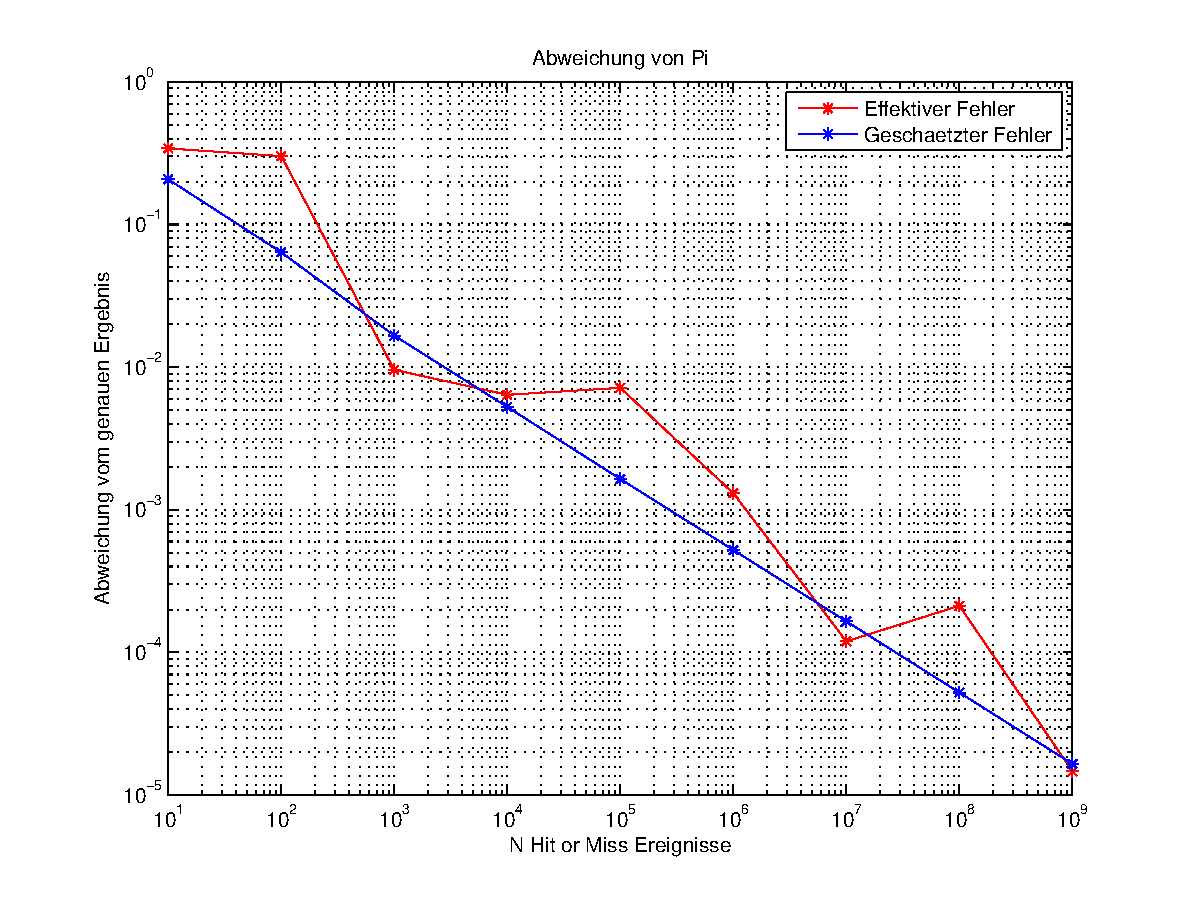
\includegraphics[width=7cm]{images/Abweichung_C.eps}
	\end{figure}
\end{frame}
\begin{frame}{Genauigkeit}
	Implementation in OpenCL
	\begin{figure}
		\centering
		\includegraphics[width=7cm]{images/Abweichung_OpenCl.eps}
	\end{figure}
\end{frame}

\section{Zufallszahlen}
\begin{frame}{Zufallszahlen}
	\begin{quote}
	\textit{“Anyone who considers arithmetical methods of producing random digits is, of course, in a state of sin.”} \\ - John von Neumann, 1951
	\end{quote}
\end{frame}

\begin{frame}{Zufallszahlen}
	Übersicht:
	\begin{itemize}
		\item<1-> Linear Congruential Generators
		\item<1-> Park-Miller Generator
		\item<1-> Mersenne-Twister Algorithmus
		\item<1-> Random Device
	\end{itemize}
\end{frame}

\subsection{Linear Congruential Generators}
\begin{frame}{Linear Congruential Generators}
	\begin{itemize}
		\item Rekursive Iterationsvorschrift: \\
				\hspace{1cm}$x_{i+1} = \left( a x_{i} + b \right) \mod{m}$ \\
				\hspace{1.5cm}$a$: Faktor\\
				\hspace{1.5cm}$b$: Inkrement\\
				\hspace{1.5cm}$m$: Modul
		\item erzeugt Zahlen zwischen $0$ und $m-1$
		\item sehr stark von Konstanten $a,b,m$ abhängig.
	\end{itemize}
\end{frame}
\begin{frame}{Linear Congruential Generators}
	\begin{figure}[h]
		\centering
		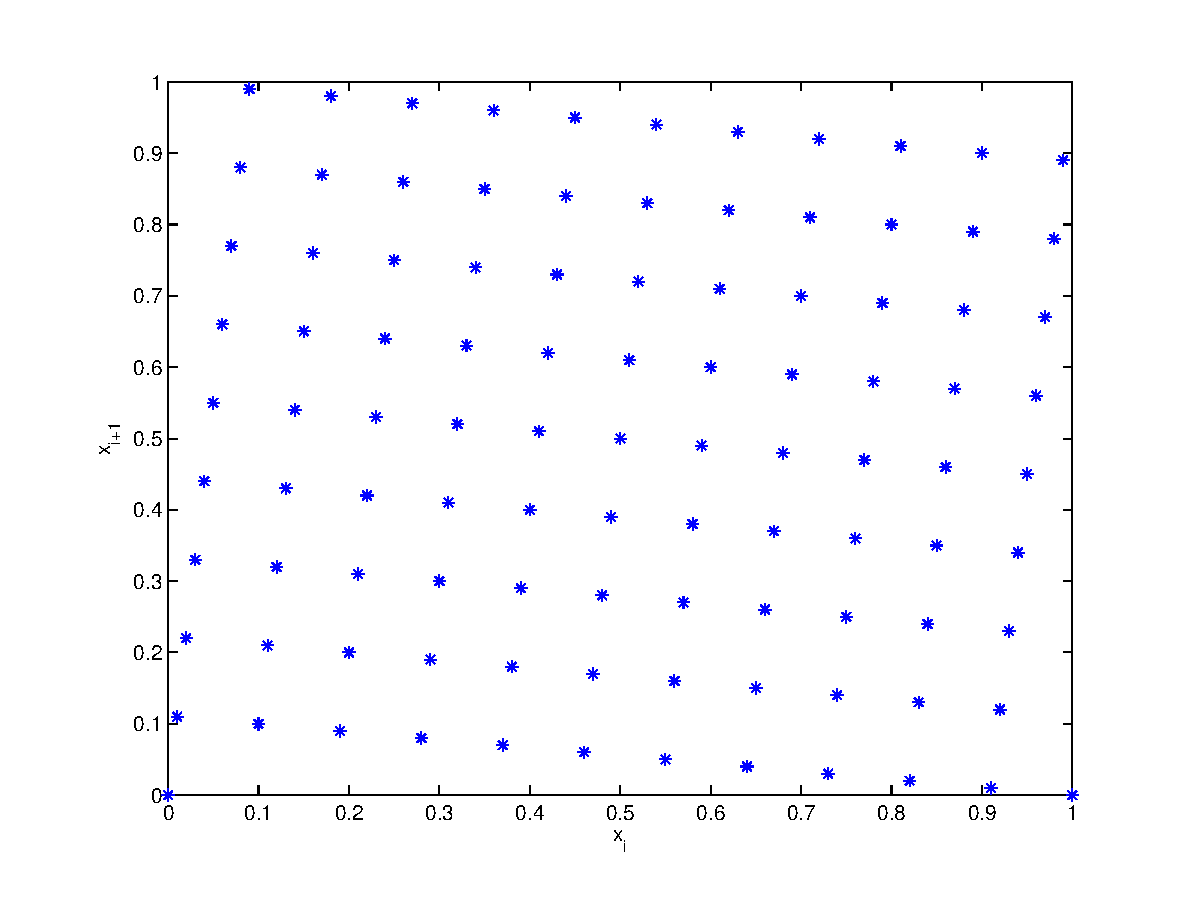
\includegraphics[width=0.7\linewidth]{images/lcg.eps}
	\end{figure}
	Verteilung aufeinanderfolgender Zufallszahlen eines LCG mit $a=11$, $b=0$, $m=64$
\end{frame}
\begin{frame}{Linear Congruential Generators}
	\begin{itemize}
		\item IBM \texttt{RANDU} Generator: in 60er Jahren Standard Random-Funktion auf IBM System/360
		\item $x_{i+1} = \left( 65539 \: x_i \right) \mod{2^{31}}$ 
		\item<4-> \textit{``really horrible''} - Donald E. Knuth.
	\end{itemize}
	\only<3>{\begin{figure}\includegraphics[width=0.75\linewidth]{images/ibm_randu.eps}\end{figure}}
\end{frame}

\subsection{Park-Miller Generator}
\begin{frame}{Park-Miller Generator}

	\begin{itemize}
		\item \texttt{rand()} Funktion von C
		\item Übliche Implementation: \\ $x_{i+1} =  \left( 1103515245 \: x_i + 12345\right) \mod{2^{31}}$
		\item Startwert mit \texttt{srand(int seed)} gesetzt. 
		\item Genaue Implementation nicht spezifiziert - gefährlich.
	\end{itemize}
\end{frame}

\begin{frame}{Park-Miller Generator}
	\begin{quote}
		\textit{Many generators have been written, most of them have demonstrably non-random characteristics, and some are embarrassingly bad.} \\ - Stephen Park, Keith Miller, 1988
	\end{quote}	
\end{frame}

\begin{frame}{Linear Congruental Generators}
	Paper von S.Park, K.Miller, 1988. \\ Ziel: neuen \textbf{Minimal Standard}
	
	\begin{itemize}
		\item<2-> $x_{i+1} = \left( 16'807 \: x_i \right) \mod{2^{31}-1}$ 
		\item<3-> Modul $m$: Primzahl $\rightarrow$ maximale Periode
		\item<4-> Faktor $a$: $7^5$ $\rightarrow$ komplett zufällige Sequenz
		\item<5-> Trotzdem einfach auf 32-bit System implementierbar.
	\end{itemize}
\end{frame}
\begin{frame}[fragile]{Park-Miller Generator}
	Einfache Implementation: \vspace{0.5cm}
	\begin{lstlisting}[style=C]
double random(int* seed) {
    const int a = 16807;
    const int m = 2147483647;
	
    *seed = (a * (*seed)) % m;
    return ((double)*seed) / m;
}
	\end{lstlisting}
	\vspace{0.5cm}
	aber...
\end{frame}
\begin{frame}{Park-Miller Generator}

	Mit $m = aq + r$ gilt:
	\begin{equation*}
		a x \text{ mod } m = 
			\begin{cases}
				a \left(x \text{ mod } q\right) - r \lfloor x / q\rfloor & \text{wenn }\geq 0 \\
				a \left(x \text{ mod } q\right) - r \lfloor x / q\rfloor + m & \text{sonst}
			\end{cases}
	\end{equation*}
\end{frame}
\begin{frame}[fragile]{Park-Miller Generator}
	Lösung: \vspace{0.5cm}
	\begin{lstlisting}[style=C]
		double random(int* seed) {
		    const int a = 16807;
		    const int m = 2147483647;
		    const int q = 127773;
		    const int r = 2836;
			
		    int k = *seed / q;
		    *seed = a * (*seed - k*q) - k*r;
		    if(*seed < 0)   *seed += m;
		    return (double)*seed / m;
		}
	\end{lstlisting}
\end{frame}

\subsection{Mersenne-Twister Algorithmus}
\begin{frame}{Mersenne-Twister Algorithmus}
	\begin{itemize}
		\item Non-Plus-Ultra der Pseudo RNGs
		\item Periode: $4.3 \cdot  10^{6001}$
		\item Bis Dimension 623 gleichverteilt
		\item 624 Zustandswörter $Y_1 \dots Y_N$
		\item $h :=  Y_{i-N} - Y_{i-N} \mod{2^{31}} + Y_{i-N+1} \mod{2^{31}}$ \\
			$Y_i := Y_{i-227} \oplus \left\lfloor \frac{h}{2} \right\rfloor \oplus \left( \left(h \mod{2} \right) \cdot 9908b0df_{\text{hex}}\right)$
		\item Trotzdem relativ schnell.
		\item Standard in \textit{GNU Scientific Library}
	\end{itemize}
\end{frame}

\subsection{Random-Device}
\begin{frame}{Random-Device}
	\begin{itemize}
		\item Bisherige RNG: Immer deterministisch, nicht für Kryptografie geeignet.
		\item Alternative: UNIX Random-Device \texttt{/dev/random} bzw. \texttt{/dev/urandom}
		\item Sammelt Rauschen von Gerätetreibern etc. in Entropiepool und generiert \textbf{echte} Zufallszahlen!
		\item Häufig als Seed für pRNGs verwendet.
	\end{itemize}
\end{frame}

\subsection[Boost]{Implementation in C++ mit Boost}
\begin{frame}{Implementation in C++ mit Boost}
	\begin{itemize}
		\item Boost: gratis C++ Source Library
		\item enthält u.a. Algorithmen, Container, Mathematik, ... 
		\item Teile bereits C++11 Standard
		\item Schöne, einfache Random-Funktionen mit:
		\begin{itemize}
			\item 30 verschiedenen RNG
			\item Verteilungsfunktionen und Wertebereiche frei wählbar
		\end{itemize}
	\end{itemize}
\end{frame}
\begin{frame}{Implementation in C++ mit Boost}
	\begin{itemize}
		\item Generator instanzieren: \\
			\texttt{static mt19937 gen(time(0));}
		\item Verteilungsfunktion wählen: \\
			\texttt{static uniform\_01 <mt19937 > dist(gen);}
		\item Fertig. \\
			\texttt{x = dist();}
	\end{itemize}
\end{frame}


\end{document}
